\documentclass{extbook}[14pt]
\usepackage{multicol, enumerate, enumitem, hyperref, color, soul, setspace, parskip, fancyhdr, amssymb, amsthm, amsmath, bbm, latexsym, units, mathtools}
\everymath{\displaystyle}
\usepackage[headsep=0.5cm,headheight=0cm, left=1 in,right= 1 in,top= 1 in,bottom= 1 in]{geometry}
\usepackage{dashrule}  % Package to use the command below to create lines between items
\newcommand{\litem}[1]{\item #1

\rule{\textwidth}{0.4pt}}
\pagestyle{fancy}
\lhead{}
\chead{Answer Key for Progress Quiz 10 Version C}
\rhead{}
\lfoot{6232-9639}
\cfoot{}
\rfoot{Fall 2020}
\begin{document}
\textbf{This key should allow you to understand why you choose the option you did (beyond just getting a question right or wrong). \href{https://xronos.clas.ufl.edu/mac1105spring2020/courseDescriptionAndMisc/Exams/LearningFromResults}{More instructions on how to use this key can be found here}.}

\textbf{If you have a suggestion to make the keys better, \href{https://forms.gle/CZkbZmPbC9XALEE88}{please fill out the short survey here}.}

\textit{Note: This key is auto-generated and may contain issues and/or errors. The keys are reviewed after each exam to ensure grading is done accurately. If there are issues (like duplicate options), they are noted in the offline gradebook. The keys are a work-in-progress to give students as many resources to improve as possible.}

\rule{\textwidth}{0.4pt}

\begin{enumerate}\litem{
Describe the end behavior of the polynomial below.
\[ f(x) = 9(x - 8)^{3}(x + 8)^{4}(x - 3)^{5}(x + 3)^{7} \]

The solution is the graph below, which is option D.
\begin{center}
    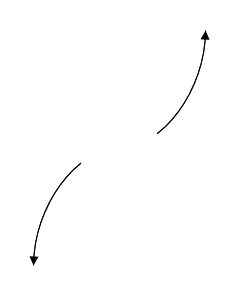
\includegraphics[width=0.3\textwidth]{../Figures/polyEndBehaviorDC.png}
\end{center}\begin{enumerate}[label=\Alph*.]
\begin{multicols}{2}
\item 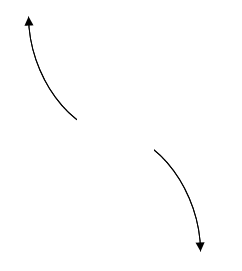
\includegraphics[width = 0.3\textwidth]{../Figures/polyEndBehaviorAC.png}
\item 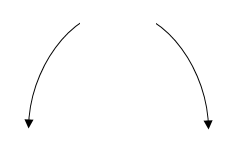
\includegraphics[width = 0.3\textwidth]{../Figures/polyEndBehaviorBC.png}
\item 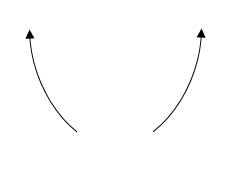
\includegraphics[width = 0.3\textwidth]{../Figures/polyEndBehaviorCC.png}
\item 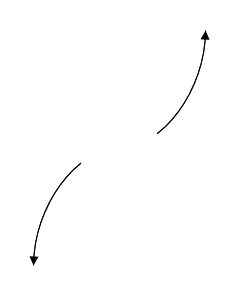
\includegraphics[width = 0.3\textwidth]{../Figures/polyEndBehaviorDC.png}
\end{multicols}\item None of the above.\end{enumerate}
\textbf{General Comment:} Remember that end behavior is determined by the leading coefficient AND whether the \textbf{sum} of the multiplicities is positive or negative.
}
\litem{
Construct the lowest-degree polynomial given the zeros below. Then, choose the intervals that contain the coefficients of the polynomial in the form $x^3+bx^2+cx+d$.
\[ -2 + 3 i \text{ and } 2 \]

The solution is \( x^{3} +2 x^{2} +5 x -26 \), which is option C.\begin{enumerate}[label=\Alph*.]
\item \( b \in [0.54, 1.25], c \in [-9, -2], \text{ and } d \in [1, 8] \)

$x^{3} + x^{2} -5 x + 6$, which corresponds to multiplying out $(x -3)(x -2)$.
\item \( b \in [0.54, 1.25], c \in [-2, 1], \text{ and } d \in [-4, 0] \)

$x^{3} + x^{2} -4$, which corresponds to multiplying out $(x + 2)(x -2)$.
\item \( b \in [1.7, 2.1], c \in [4, 7], \text{ and } d \in [-29, -22] \)

* $x^{3} +2 x^{2} +5 x -26$, which is the correct option.
\item \( b \in [-2.25, -0.75], c \in [4, 7], \text{ and } d \in [25, 29] \)

$x^{3} -2 x^{2} +5 x + 26$, which corresponds to multiplying out $(x-(-2 + 3 i))(x-(-2 - 3 i))(x + 2)$.
\item \( \text{None of the above.} \)

This corresponds to making an unanticipated error or not understanding how to use nonreal complex numbers to create the lowest-degree polynomial. If you chose this and are not sure what you did wrong, please contact the coordinator for help.
\end{enumerate}

\textbf{General Comment:} Remember that the conjugate of $a+bi$ is $a-bi$. Since these zeros always come in pairs, we need to multiply out $(x-(-2 + 3 i))(x-(-2 - 3 i))(x-(2))$.
}
\litem{
Describe the zero behavior of the zero $x = 2$ of the polynomial below.
\[ f(x) = -8(x - 2)^{9}(x + 2)^{12}(x + 6)^{7}(x - 6)^{9} \]

The solution is the graph below, which is option D.
\begin{center}
    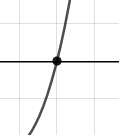
\includegraphics[width=0.3\textwidth]{../Figures/polyZeroBehaviorCopyDC.png}
\end{center}\begin{enumerate}[label=\Alph*.]
\begin{multicols}{2}
\item 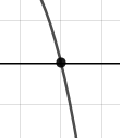
\includegraphics[width = 0.3\textwidth]{../Figures/polyZeroBehaviorCopyAC.png}
\item 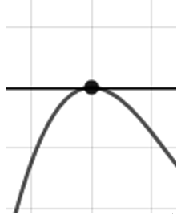
\includegraphics[width = 0.3\textwidth]{../Figures/polyZeroBehaviorCopyBC.png}
\item 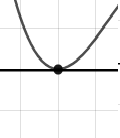
\includegraphics[width = 0.3\textwidth]{../Figures/polyZeroBehaviorCopyCC.png}
\item 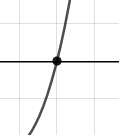
\includegraphics[width = 0.3\textwidth]{../Figures/polyZeroBehaviorCopyDC.png}
\end{multicols}\item None of the above.\end{enumerate}
\textbf{General Comment:} You will need to sketch the entire graph, then zoom in on the zero the question asks about.
}
\litem{
Construct the lowest-degree polynomial given the zeros below. Then, choose the intervals that contain the coefficients of the polynomial in the form $ax^3+bx^2+cx+d$.
\[ \frac{6}{5}, \frac{-1}{3}, \text{ and } \frac{2}{5} \]

The solution is \( 75x^{3} -95 x^{2} -4 x + 12 \), which is option B.\begin{enumerate}[label=\Alph*.]
\item \( a \in [70, 82], b \in [34, 42], c \in [-60, -51], \text{ and } d \in [10, 14] \)

$75x^{3} +35 x^{2} -56 x + 12$, which corresponds to multiplying out $(5x + 6)(3x -1)(5x -2)$.
\item \( a \in [70, 82], b \in [-103, -90], c \in [-5, -2], \text{ and } d \in [10, 14] \)

* $75x^{3} -95 x^{2} -4 x + 12$, which is the correct option.
\item \( a \in [70, 82], b \in [91, 96], c \in [-5, -2], \text{ and } d \in [-15, -9] \)

$75x^{3} +95 x^{2} -4 x -12$, which corresponds to multiplying out $(5x + 6)(3x -1)(5x + 2)$.
\item \( a \in [70, 82], b \in [-103, -90], c \in [-5, -2], \text{ and } d \in [-15, -9] \)

$75x^{3} -95 x^{2} -4 x -12$, which corresponds to multiplying everything correctly except the constant term.
\item \( a \in [70, 82], b \in [78, 91], c \in [-17, -13], \text{ and } d \in [-15, -9] \)

$75x^{3} +85 x^{2} -16 x -12$, which corresponds to multiplying out $(5x + 6)(3x + 1)(5x -2)$.
\end{enumerate}

\textbf{General Comment:} To construct the lowest-degree polynomial, you want to multiply out $(5x -6)(3x + 1)(5x -2)$
}
\litem{
Which of the following equations \textit{could} be of the graph presented below?

\begin{center}
    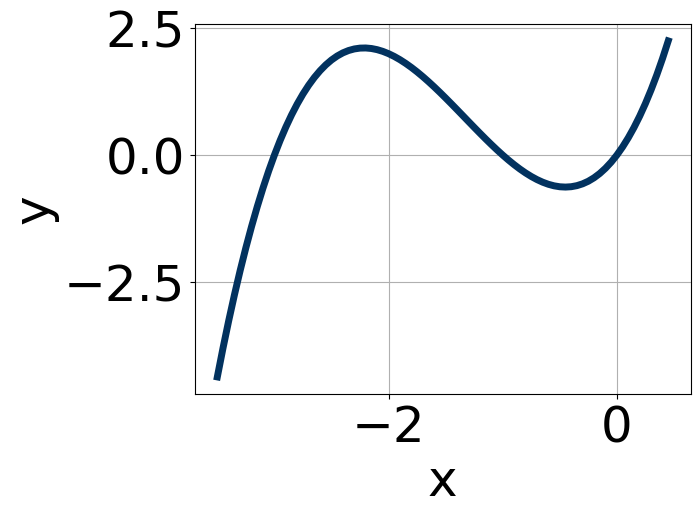
\includegraphics[width=0.5\textwidth]{../Figures/polyGraphToFunctionC.png}
\end{center}




The solution is \( 15x^{5} (x + 3)^{5} (x + 1)^{5} \), which is option A.\begin{enumerate}[label=\Alph*.]
\item \( 15x^{5} (x + 3)^{5} (x + 1)^{5} \)

* This is the correct option.
\item \( 11x^{9} (x + 3)^{4} (x + 1)^{9} \)

The factor $-3$ should have been an odd power.
\item \( 12x^{7} (x + 3)^{4} (x + 1)^{6} \)

The factors $-3$ and $-1$ have have been odd power.
\item \( -19x^{5} (x + 3)^{10} (x + 1)^{9} \)

The factor $(x + 3)$ should have an odd power and the leading coefficient should be the opposite sign.
\item \( -9x^{7} (x + 3)^{11} (x + 1)^{7} \)

This corresponds to the leading coefficient being the opposite value than it should be.
\end{enumerate}

\textbf{General Comment:} General Comments: Draw the x-axis to determine which zeros are touching (and so have even multiplicity) or cross (and have odd multiplicity).
}
\litem{
Describe the zero behavior of the zero $x = -4$ of the polynomial below.
\[ f(x) = 4(x + 4)^{8}(x - 4)^{13}(x + 9)^{7}(x - 9)^{8} \]

The solution is the graph below, which is option B.
\begin{center}
    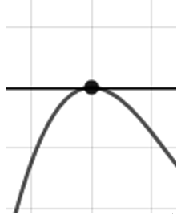
\includegraphics[width=0.3\textwidth]{../Figures/polyZeroBehaviorBC.png}
\end{center}\begin{enumerate}[label=\Alph*.]
\begin{multicols}{2}
\item 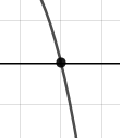
\includegraphics[width = 0.3\textwidth]{../Figures/polyZeroBehaviorAC.png}
\item 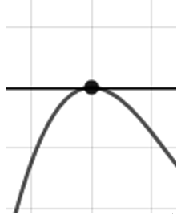
\includegraphics[width = 0.3\textwidth]{../Figures/polyZeroBehaviorBC.png}
\item 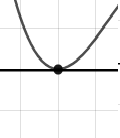
\includegraphics[width = 0.3\textwidth]{../Figures/polyZeroBehaviorCC.png}
\item 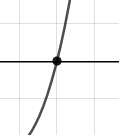
\includegraphics[width = 0.3\textwidth]{../Figures/polyZeroBehaviorDC.png}
\end{multicols}\item None of the above.\end{enumerate}
\textbf{General Comment:} You will need to sketch the entire graph, then zoom in on the zero the question asks about.
}
\litem{
Describe the end behavior of the polynomial below.
\[ f(x) = -7(x + 2)^{4}(x - 2)^{7}(x + 9)^{4}(x - 9)^{6} \]

The solution is the graph below, which is option A.
\begin{center}
    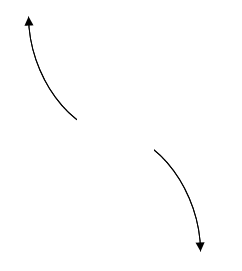
\includegraphics[width=0.3\textwidth]{../Figures/polyEndBehaviorCopyAC.png}
\end{center}\begin{enumerate}[label=\Alph*.]
\begin{multicols}{2}
\item 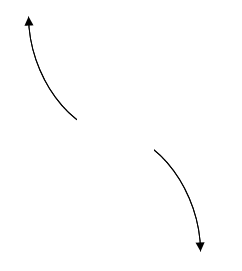
\includegraphics[width = 0.3\textwidth]{../Figures/polyEndBehaviorCopyAC.png}
\item 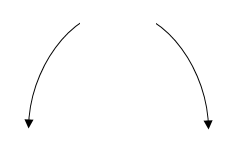
\includegraphics[width = 0.3\textwidth]{../Figures/polyEndBehaviorCopyBC.png}
\item 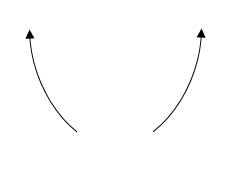
\includegraphics[width = 0.3\textwidth]{../Figures/polyEndBehaviorCopyCC.png}
\item 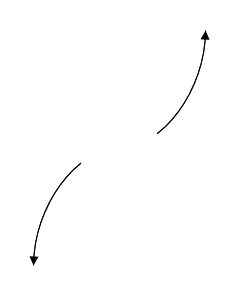
\includegraphics[width = 0.3\textwidth]{../Figures/polyEndBehaviorCopyDC.png}
\end{multicols}\item None of the above.\end{enumerate}
\textbf{General Comment:} Remember that end behavior is determined by the leading coefficient AND whether the \textbf{sum} of the multiplicities is positive or negative.
}
\litem{
Construct the lowest-degree polynomial given the zeros below. Then, choose the intervals that contain the coefficients of the polynomial in the form $x^3+bx^2+cx+d$.
\[ 3 + 5 i \text{ and } -3 \]

The solution is \( x^{3} -3 x^{2} +16 x + 102 \), which is option C.\begin{enumerate}[label=\Alph*.]
\item \( b \in [2.51, 4.34], c \in [15.82, 16.89], \text{ and } d \in [-103.2, -101.1] \)

$x^{3} +3 x^{2} +16 x -102$, which corresponds to multiplying out $(x-(3 + 5 i))(x-(3 - 5 i))(x -3)$.
\item \( b \in [-1.5, 2.17], c \in [-1.04, 0.81], \text{ and } d \in [-9.6, -7.5] \)

$x^{3} + x^{2} -9$, which corresponds to multiplying out $(x -3)(x + 3)$.
\item \( b \in [-4.81, -1.83], c \in [15.82, 16.89], \text{ and } d \in [99.1, 105] \)

* $x^{3} -3 x^{2} +16 x + 102$, which is the correct option.
\item \( b \in [-1.5, 2.17], c \in [-2.18, -1.34], \text{ and } d \in [-19.2, -13.9] \)

$x^{3} + x^{2} -2 x -15$, which corresponds to multiplying out $(x -5)(x + 3)$.
\item \( \text{None of the above.} \)

This corresponds to making an unanticipated error or not understanding how to use nonreal complex numbers to create the lowest-degree polynomial. If you chose this and are not sure what you did wrong, please contact the coordinator for help.
\end{enumerate}

\textbf{General Comment:} Remember that the conjugate of $a+bi$ is $a-bi$. Since these zeros always come in pairs, we need to multiply out $(x-(3 + 5 i))(x-(3 - 5 i))(x-(-3))$.
}
\litem{
Which of the following equations \textit{could} be of the graph presented below?

\begin{center}
    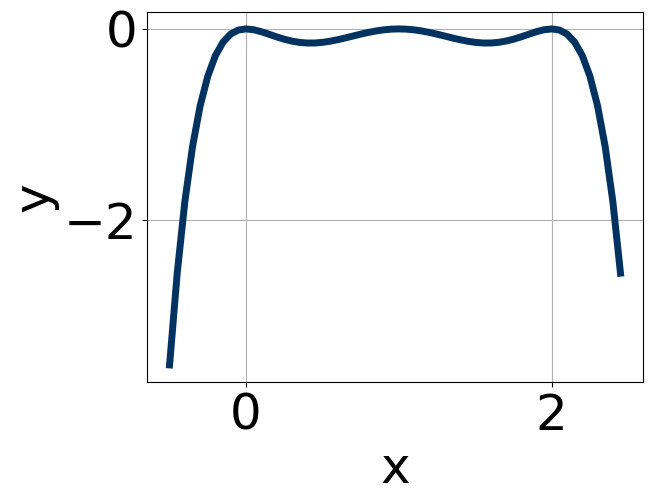
\includegraphics[width=0.5\textwidth]{../Figures/polyGraphToFunctionCopyC.png}
\end{center}




The solution is \( -17x^{6} (x - 2)^{8} (x - 1)^{4} \), which is option A.\begin{enumerate}[label=\Alph*.]
\item \( -17x^{6} (x - 2)^{8} (x - 1)^{4} \)

* This is the correct option.
\item \( -16x^{8} (x - 2)^{4} (x - 1)^{11} \)

The factor $(x - 1)$ should have an even power.
\item \( 13x^{8} (x - 2)^{8} (x - 1)^{11} \)

The factor $(x - 1)$ should have an even power and the leading coefficient should be the opposite sign.
\item \( 18x^{8} (x - 2)^{6} (x - 1)^{4} \)

This corresponds to the leading coefficient being the opposite value than it should be.
\item \( -2x^{8} (x - 2)^{5} (x - 1)^{7} \)

The factors $(x - 2)$ and $(x - 1)$ should both have even powers.
\end{enumerate}

\textbf{General Comment:} General Comments: Draw the x-axis to determine which zeros are touching (and so have even multiplicity) or cross (and have odd multiplicity).
}
\litem{
Construct the lowest-degree polynomial given the zeros below. Then, choose the intervals that contain the coefficients of the polynomial in the form $ax^3+bx^2+cx+d$.
\[ -4, \frac{3}{5}, \text{ and } \frac{5}{3} \]

The solution is \( 15x^{3} +26 x^{2} -121 x + 60 \), which is option B.\begin{enumerate}[label=\Alph*.]
\item \( a \in [14, 16], b \in [-94, -92], c \in [149, 155], \text{ and } d \in [-66, -56] \)

$15x^{3} -94 x^{2} +151 x -60$, which corresponds to multiplying out $(x -4)(5x -3)(3x -5)$.
\item \( a \in [14, 16], b \in [20, 30], c \in [-121, -118], \text{ and } d \in [53, 62] \)

* $15x^{3} +26 x^{2} -121 x + 60$, which is the correct option.
\item \( a \in [14, 16], b \in [20, 30], c \in [-121, -118], \text{ and } d \in [-66, -56] \)

$15x^{3} +26 x^{2} -121 x -60$, which corresponds to multiplying everything correctly except the constant term.
\item \( a \in [14, 16], b \in [-83, -73], c \in [46, 50], \text{ and } d \in [53, 62] \)

$15x^{3} -76 x^{2} +49 x + 60$, which corresponds to multiplying out $(x -4)(5x + 3)(3x -5)$.
\item \( a \in [14, 16], b \in [-29, -22], c \in [-121, -118], \text{ and } d \in [-66, -56] \)

$15x^{3} -26 x^{2} -121 x -60$, which corresponds to multiplying out $(x -4)(5x + 3)(3x + 5)$.
\end{enumerate}

\textbf{General Comment:} To construct the lowest-degree polynomial, you want to multiply out $(x + 4)(5x -3)(3x -5)$
}
\end{enumerate}

\end{document}